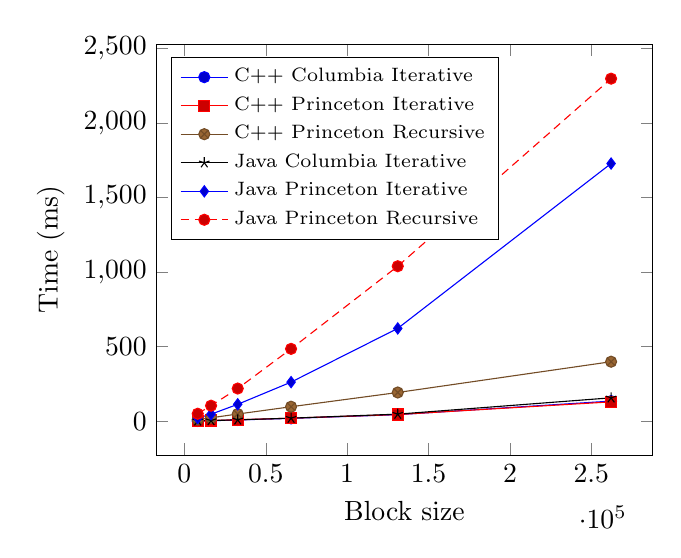
\begin{tikzpicture}
\begin{axis}[xlabel={Block size},ylabel={Time (ms)},width=0.65\linewidth,legend pos=north west,scaled y ticks = false,legend cell align=left,legend style={font=\scriptsize}]
\addplot coordinates {
(8192, 1.8030)
(16384, 2.9629)
(32768, 8.2847)
(65536, 18.8158)
(131072, 43.7807)
(262144, 134.8093)
};
\addplot coordinates {
(8192, 2.0605)
(16384, 4.5027)
(32768, 9.6797)
(65536, 20.3049)
(131072, 44.5770)
(262144, 129.5150)
};
\addplot coordinates {
(8192, 10.7496)
(16384, 22.8640)
(32768, 48.0022)
(65536, 96.9572)
(131072, 192.4607)
(262144, 398.9698)
};
\addplot coordinates {
(8192, 2.1766)
(16384, 3.9995)
(32768, 8.9846)
(65536, 20.2833)
(131072, 47.2950)
(262144, 156.7135)
};
\addplot coordinates {
(8192, 21.1757)
(16384, 46.8150)
(32768, 113.1953)
(65536, 261.9954)
(131072, 622.4328)
(262144, 1728.4640)
};
\addplot coordinates {
(8192, 50.0776)
(16384, 103.9682)
(32768, 219.0208)
(65536, 485.1020)
(131072, 1039.4937)
(262144, 2297.8011)
};
\legend{C++ Columbia Iterative,C++ Princeton Iterative,C++ Princeton Recursive,Java Columbia Iterative,Java Princeton Iterative,Java Princeton Recursive}
\end{axis}
\end{tikzpicture}
